%%%%%%%%%%%%%%%%%%%%%%%%%%%%%%%%%%%%%%%%%%%%%%%%%%%%%%%%%%%%%%%%%%%%%%%%%%%%%%%%
% PhD Thesis Defense
% Giovanni Ciatto
% Alma Mater Studiorum - Università di Bologna
% mailto:giovanni.ciatto@unibo.it
%%%%%%%%%%%%%%%%%%%%%%%%%%%%%%%%%%%%%%%%%%%%%%%%%%%%%%%%%%%%%%%%%%%%%%%%%%%%%%%%
%\documentclass[handout]{beamer}\mode<handout>{\usetheme{default}}
%
\documentclass[presentation]{beamer}\mode<presentation>{\usetheme{AMSBolognaFC}}
%\documentclass[handout]{beamer}\mode<handout>{\usetheme{AMSBolognaFC}}
%%%%%%%%%%%%%%%%%%%%%%%%%%%%%%%%%%%%%%%%%%%%%%%%%%%%%%%%%%%%%%%%%%%%%%%%%%%%%%%%
\usepackage{phd-defense}
% version
\newcommand{\versionmajor}{1}
\newcommand{\versionminor}{0}
\newcommand{\versionpatch}{2}
\version{\versionmajor.\versionminor.\versionpatch}
%%%%%%%%%%%%%%%%%%%%%%%%%%%%%%%%%%%%%%%%%%%%%%%%%%%%%%%%%%%%%%%%%%%%%%%%%%%%%%%%

\school{\unibo}
%
\schoolShort{\uniboShort}
%
\programme{PhD Programme in `Data Science and Computation'}
%
\programmeShort{DS\&C}
%
\title[Role of CL in DS]{On the role of Computational Logic in Data Science}
%
\subtitle{Representing, Learning, Reasoning, and Explaining Knowledge}
%
\candidate{Giovanni Ciatto}
\candidateShort{G. Ciatto}
\candidateEmail{giovanni.ciatto@unibo.it}
%
\supervisor{Prof. Andrea Omicini}
\supervisorShort{A. Omicini}
\supervisorEmail{andrea.omicini@unibo.it}
%
\coordinator{Prof. Andrea Cavalli}
\coordinatorShort{A. Cavalli}
\coordinatorEmail{andrea.cavalli@unibo.it}
%
\contestsector{09/H1 -- Sistemi di Elaborazione delle Informazioni}
%
\scientificsector{ING-INF/05 -- Sistemi di Elaborazione delle Informazioni}
%
\cycle{XXXIII}
%
\examdate{June 16, 2022}
%
\examdateShort{2022-06-16}

\makeinfo

%%%%%%%%%%%%%%%%%%%%%%%%%%%%%%%%%%%%%%%%%%%%%%%%%%%%%%%%%%%%%%%%%%%%%%%%%%%%%%%%
\begin{document}
%%%%%%%%%%%%%%%%%%%%%%%%%%%%%%%%%%%%%%%%%%%%%%%%%%%%%%%%%%%%%%%%%%%%%%%%%%%%%%%%

%/////////
\frame{\titlepage}
%/////////

%%===============================================================================
\section*{Outline}
%%===============================================================================
%
%%/////////
\frame[c]{\tableofcontents[hideallsubsections]}
%%/////////

%===============================================================================
\section{Candidate Presentation}
%===============================================================================

\begin{frame}{About Me \hfill \uurl{https://about.me/gciatto}}
    \begin{itemize}
        \item Bachelor in \alert{Software Engineering} (2011--2014)

        \vfill
        
        \item Master in \alert{Computer Science and Engineering} (2014--2017)

        \vfill
        
        \item PhD in \alert{Data Science and Computation} (2017--2022)
        %
        \begin{itemize}
            \item with a focus on foundational \alert{Artificial Intelligence}
        \end{itemize}

        \vfill
        
        \item Currently:
        %
        \begin{itemize}
            \item research fellow at \disiShort{} (\uniboShort{})
            \item funded by the \alert{EXPECTATION} project\footnote{\url{http://www.chistera.eu/projects/expectation}}
            %
            \begin{itemize}
                \item where I am WP-leader
            \end{itemize}
        \end{itemize}
    \end{itemize}
\end{frame}

%===============================================================================
\section{Context, Motivation, and Goals}
%===============================================================================

\begin{frame}{Context}
    \begin{itemize}
        \item Era of \alert{data-driven} artificial intelligence (AI)
        %
        \begin{itemize}
            \item major availability of \alert{data} and \alert{computational resources}
            \item pervasive exploitation in science and in the industry
        \end{itemize}

        \vfill

        \item Deep entanglement among AI and \alert{data science} (DS)
        %
        \begin{itemize}
            \item both leveraging \alert{machine learning} to mine information from data
        \end{itemize}
        
        \vfill

        \item AI involves not only data-driven approaches
        %
        \begin{itemize}
            \item[eg] good old-fashioned AI (GOFAI), \alert{computational logic}\ccite{lloyd1990computational} (CL) 
        \end{itemize}

        \vfill
        
        \item Following a ``classical'' perspective, we distinguish among\ccite{explanation-aixia2020dp}
        %
        \begin{itemize}
            \item \alert{symbolic} AI $\approx$ CL $\rightarrow$ emulating humans' \alert{rational reasoning}
            \item \alert{\emph{sub}-symbolic} $\approx$ ML / DS  $\rightarrow$ emulating humans' \alert{intuition}
        \end{itemize}
    \end{itemize}
\end{frame}

\begin{frame}{Motivation}
    \begin{itemize}
        \item \alert{Limitation} of sub-symbolic AI are now becoming relevant \alert{issues}, e.g.
        %
        \begin{itemize}
            \item interpretability/\alert{explainability}\ccite{darpa2016-xai}
            \item data-greediness\ccite{CropperDM20}
            \item human-in-the-loop\ccite{Yao2018}
        \end{itemize}
        
        \vfill

        \item Symbolic and sub-symbolic have several \alert{complementarities}
        %
        \begin{itemize}
            \item[$\rightarrow$] integrating the two may lead to a better AI\ccite{Hoehndorf2017}
        \end{itemize}

        \vfill

        \item Long-standing interest in \alert{integrating} the two\ccite{IlkouK20}

        \vfill

        \item Interest in spotting (and overcoming) \alert{obstacles} preventing integration
        %
        \begin{itemize}
            \item either at the theoretical or technological level
        \end{itemize}
    \end{itemize}
\end{frame}

\begin{frame}{Goals}

    \emph{Foundational} goals:
    %
    \vfill
    %
    \begin{enumerate}
        \item \alert{comparing} DS and CL w.r.t. how they manage \alert{knowledge}
        %
        \begin{itemize}
            \item \alert{representation}
            \item acquisition (a.k.a. \alert{learning})
            \item inference (a.k.a. \alert{reasoning})
            \item transferring (a.k.a. \alert{explanation})
        \end{itemize}
        
        \vfill

        \item \alert{elicit} synergies and complementarities, and frictions w.r.t. \alert{integration}

        \vfill

        \item assess the \alert{technological gap} among the two
        %
        \begin{itemize}
            \item design \& \alert{prototype software} technologies for filling it
        \end{itemize}
    \end{enumerate}
\end{frame}

\begin{frame}{Organization of the Thesis}

    Two major parts, concerning the integration of CL and DS:
    %
    \vfill
    %
    \begin{block}{\textbf{Computational} perspective: \textbf{what} aspects can be integreted}
        \begin{enumerate}
            \item understand the \alert{analogies} and \alert{differences} among CL and DS
            \item derive a \alert{conceptual framework} bridging them
        \end{enumerate}
    \end{block}
    %
    \vfill
    %
    \begin{block}{\textbf{Technological} perspective: \textbf{how} to integrate them}
        \begin{enumerate}\setcounter{enumi}{2}
            \item evaluate the current \alert{state of the art} of AI \alert{technologies}
            \item propose the notion of \alert{logic ecosystem} to support integration
            \item discuss the \alert{reification} of logic ecosystems into \alert{software}
        \end{enumerate}
    \end{block}

\end{frame}

%===============================================================================
\section{Background}
%===============================================================================

% \subsection{Data Science}

\begin{frame}{Data Science\ccite{Hoehndorf2017}}
    \begin{itemize}
        \item Novel discipline laying at the intersection among \ldots
        %
        \begin{itemize}
            \item[] \ldots Computer Science, Statistics, AI, Software Engineering
        \end{itemize}
        
        \vfill 
        
        \item Focus on modelling the world following a \alert{data-driven} approach
        %
        \begin{itemize}
            \item possibly, by leveraging \alert{Machine Learning} (ML) or Data Mining
        \end{itemize}
        
        \vfill

        \item Pros/cons:
        %
        \begin{itemize}
            \item[$+$] data-driven $\rightarrow$ \alert{bottom-up} $\rightarrow$ adherence to reality
            \item[$+$] \alert{scalable} algorithms for learning
            \item[$\sim$] \alert{flexibility} w.r.t. errors in the data or in the model
            \item[$-$] reliance on \alert{poorly interpretable} models
            \item[$-$] simple, \alert{stimulus--response} form of inference
        \end{itemize}
    \end{itemize}
\end{frame}

% \subsection{Computational Logic}

\begin{frame}{Computational Logic\ccite{lloyd1990computational}}
    \begin{itemize}
        \item Well-established discipline laying at the intersection among\ldots
        %
        \begin{itemize}
            \item[] \ldots Computer Science, Logic, and Mathematics
        \end{itemize} 
        
        \vfill 
        
        \item Focus on using \alert{formal logics} as means for \alert{computing}
        %
        \begin{itemize}
            \item hence, on making software systems able to \alert{reason}, automatically
        \end{itemize}
        
        \vfill

        \item Pros/cons:
        %
        \begin{itemize}
            \item[$+$] powerful, ``\alert{rational}'' form of inference
            \item[$+$] reliance on machine- and human-\alert{interpretable} representations
            \item[$\sim$] \alert{crisp} and \alert{exact} representations and decisions
            \item[$-$] reliance on poorly scalable, \alert{often untractable}, or undecidable algorithms
            \item[$-$] \alert{top-down} approach to knowledge, possibly detached from reality
        \end{itemize}
    \end{itemize}
\end{frame}

%===============================================================================
\section{Computational Perspective (What)}
%===============================================================================

\begin{frame}{Overview}
    Four major aspects to be analysed:
    %
    \vfill
    %
    \begin{description}
        \item[Representation:] how are data and knowledge \alert{expressed}
        %
        \begin{itemize}
            \item[\ldots] and made available to computers / humans
        \end{itemize}
        
        \vfill

        \item[Learning:] how is novel re-usable knowledge \alert{distilled} from data
        
        \vfill

        \item[Inference:] how are predictions \alert{drawn} from prior knowledge
        
        \vfill

        \item[Explanation:] how is information \alert{transferred} to another (human?) agent

    \end{description}
\end{frame}

\subsection{Representation}

\begin{frame}[allowframebreaks]{CL vs. DS -- Representation}
    \begin{block}{DS leverages on \textbf{sub-symbolic} representations}
        \begin{itemize}
            \item $\begin{cases}
                \alert{\text{data}} \rightarrow \text{numeric datasets of \alert{fixed} size}
                \\
                \alert{\text{knowledge}} \rightarrow \text{\alert{opaque} models mimicking \alert{real functions}}
            \end{cases}$
            \item issues may arise from \alert{recursive}, or \alert{depth-unlimited} concepts
            \item representations may easily become \alert{unintelligible} 
        \end{itemize}
    \end{block}

    \begin{block}{CL leverages on \textbf{symbolic} formulae}
        \begin{itemize}
            \item several \alert{logic formalisms} available
            \begin{itemize}
                \item \alert{expressivity--tractability} trade-off\ccite{LevesqueB87}
                \item good trade-off\ccite{Makowsky1987} provided by \alert{Horn clauses}\ccite{Horn1951}
            \end{itemize}
            \item coherent representation of \alert{both} data and knowledge via relations
            \item both human- and machine-\alert{interpretable}
            \item support for \alert{intensional} representations
            \item support for \alert{recursive} / structured information
            \end{itemize}
    \end{block}
\end{frame}

\begin{frame}{What does `symbolic' actually mean?}
    \begin{block}{\textbf{Symbolic} representations of knowledge should\cccite{Gelder90}}
        \begin{itemize}
            \item involve a \alert{set of symbols},
            \item which can be combined in (possibly) \alert{infinitely many} ways, 
            \item following precise \alert{syntactical} rules, and
            \item where both elementary and combined symbols have \alert{meaning}
            %
            \begin{itemize}
                \item[ie] \alert{each} symbol can be mapped into some entity from the domain at hand.
            \end{itemize}
        \end{itemize}
    \end{block}

    \begin{alertblock}{Opposite notion: \textit{distributed} representations (a.k.a. \textbf{sub-symbolic})}
        \begin{itemize}
            \item where symbols \alert{alone} have no meaning\ldots
            \item \ldots unless it is considered along with its \alert{neighbourhood}
            %
            \begin{itemize}
                \item[ie] any other symbol which is \alert{close} (according to some notion of closeness)
            \end{itemize}
        \end{itemize}
    \end{alertblock}
\end{frame}

\subsection{Learning}

\begin{frame}[allowframebreaks]{CL vs. DS -- Learning}
    \begin{block}{Similar formulation}
        \begin{itemize}
            \item \alert{search} the best hypothesis in the \alert{hypothesis space} ($\mathcal{H}$)
            \item \alert{human-in-the-loop} required to choose the $\mathcal{H}$
            \item automatic procedures for \alert{exploring} the $\mathcal{H}$
            \item learning as \alert{non-deterministic} (possibly stochastic) process
        \end{itemize}
    \end{block}

    \begin{block}{Different implementations}
        \begin{itemize}
            \item DS $\rightarrow$ numeric data $\rightarrow$ $\mathcal{H}$ is \alert{differentiable}
            %
            \begin{itemize}
                \item search by \alert{gradient descent}
                \item \alert{fuzzy} constraints, fuzzy outcomes
                \item support for \alert{hardware acceleration} via TPU
            \end{itemize}

            \bigskip

            \item CL $\rightarrow$ symbolic knowledge bases $\rightarrow$ $\mathcal{H}$ is \alert{discrete}
            %
            \begin{itemize}
                \item search by \alert{inductive logic programming}\ccite{CropperD2020}
                \item \alert{crisp} constraints, consistent outcomes
                \item \emph{virtual} support for \alert{concurrency} \hint{unexplored}
            \end{itemize}
        \end{itemize}
    \end{block}

    \begin{block}{Different expectations}
        \begin{itemize}
            \item DS learns numeric \alert{functions}
            \item CL learns symbolic \alert{relations}, in the form of \alert{logic programs}
            %
            \begin{itemize}
                \item possibly \alert{recursive}, \alert{intelligible}, and expressive
            \end{itemize}
        \end{itemize}
    \end{block}
\end{frame}

\begin{frame}{Inductive Logic Programming Example}
    \prologimport{listings/ilp-example.pl}
    %
    \begin{exampleblock}{Here the goal is \textbf{inducing} the theory}
        \begin{itemize}
            \item \prolog{grand_parent(X, Y) :- parent(X, Z), parent(Z, Y).}
        \end{itemize}
    \end{exampleblock}
\end{frame}

\subsection{Inference}

\begin{frame}%[allowframebreaks]
    \frametitle{CL vs. DS -- Inference}

    \begin{block}{DS feeds trained models with unseen data}
        \begin{itemize}
            \item \alert{inference} $\approx$ quick \& dirty responses to stimuli
            \item models as black-box functions
        \end{itemize}
    \end{block}

    \begin{block}{CL applies inference rules in a principled way}
        \begin{itemize}
            \item \alert{inference} $\approx$ reasoning $\approx$ drawing conclusions from prior knowledge 
            \item several ways of reasoning:
            %
            \begin{itemize}
                \item deductive, e.g. SLD\ccite{Kowalski1976} and Prolog\ccite{Korner2020HistoryFuturePrologTPLP}
                \item inductive, e.g. ILP\ccite{CropperDM20}
                \item abductive, e.g. IFF\ccite{FungK97}
                \item probabilistic, e.g. LPAD\ccite{VennekensVB04} 
            \end{itemize}
            \item reasoners as expert \alert{oracles} to be queried 
            %
            % \begin{itemize}
            %     \item users may either observe the result or the reasoning process
            % \end{itemize}
            \item reasoning may involve \alert{Turing-complete} computations
            %
            \begin{itemize}
                \item[$\implies$] requires computational \alert{time/space}
            \end{itemize}
        \end{itemize}
    \end{block}
\end{frame}

\subsection{Explanation}

\begin{frame}%[allowframebreaks]
    \frametitle{CL vs. DS -- Explaining}

    \begin{block}{The \textbf{opacity} problem in ML}
        \begin{itemize}
            \item due to sub-symbolic models being \alert{black boxes}\ccite{Lipton18}
            \item need to \alert{explain} how they work $\rightarrow$ \alert{eXplanable AI} (XAI)\ccite{darpa2016-xai}
        \end{itemize}
    \end{block}

    \begin{alertblock}{\textbf{Symbolic} systems are inherently \textbf{interpretable}}
        \begin{itemize}
            \item as \alert{symbols} are meant to \alert{carry meaning} for users
            \item insight: \alert{convert} sub-symbolic models into symbolic ones
        \end{itemize}
    \end{alertblock}
\end{frame}

\begin{frame}%[allowframebreaks]
    \frametitle{An Abstract Framework for XAI\ccite{agentbasedxai-extraamas2020}}

    \begin{center}
        \includegraphics[width=.5\linewidth]{figures/framework.pdf}
    \end{center}
    %
    % \begin{itemize}
    %     \item[$X$] object to be explained
    %     \item[$A$] observer agent
    %     \item[$I_A(\cdot)$] a function ``measuring'' the ``degree of interpretability'' of $X$, w.r.t. $A$
    %     \item[$E(\cdot)$] an \alert{explanation} function, mapping objects into (different) objects      
    %     \item[$X'$] the \alert{result} of the explanation, i.e. a \alert{more-interpretable} object
    % \end{itemize}
    
    \begin{block}{Key points}
        \begin{itemize}
            \item interpretation is \alert{subjective}
            \item explanation $\approx$ search of a \alert{more interpretable} model
        \end{itemize}
    \end{block}
\end{frame}

\begin{frame}[allowframebreaks]{Symbolic Knowledge Extraction (SKE)}
    \begin{columns}
        \begin{column}{0.19\linewidth}
            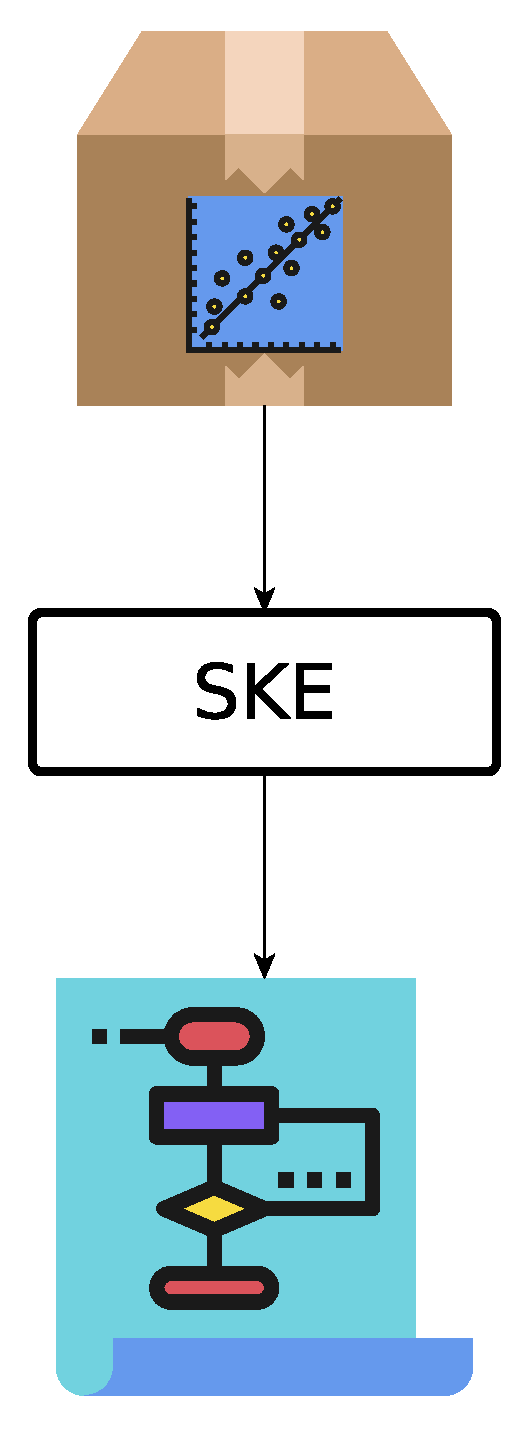
\includegraphics[width=\linewidth]{figures/ske.pdf}
        \end{column}
        \hfill
        \begin{column}{0.8\linewidth}
            \begin{block}{Insight}
                \begin{itemize}
                    \item search of a \alert{surrogate} interpretable model\ldots
                    \medskip
                    \item \ldots consisting of \alert{symbolic knowledge}
                \end{itemize}
            \end{block}
        \end{column}
    \end{columns}

    \framebreak

    Example:
    %
    \begin{columns}
        \begin{column}{.43\linewidth}
            \fbox{\includegraphics[width=\linewidth]{figures/nn-iris.png}}
        \end{column}
        %
        \begin{column}{.53\linewidth}\small
            \[ 
                \begin{array}{l}
                    \variable{Class} = \functor{setosa} \leftarrow \variable{PetalWidth} \leq 1.0 \fullstop
                    \\
                    \\
                    \variable{Class} = \functor{versicolor} \leftarrow \variable{PetalLength} > 4.9 \\ 
                        \qquad  \wedge\ \variable{SepalWidth} \in [2.9,\ 3.2] \fullstop
                    \\
                    \variable{Class} = \functor{versicolor} \leftarrow  \variable{PetalWidth} > 1.6 \fullstop
                    \\
                    \\
                    \variable{Class} = \functor{virginica} \leftarrow \variable{SepalWidth} \leq 2.9 \fullstop
                    \\
                    \\
                    \variable{Class} = \functor{virginica} \leftarrow \\ 
                        \qquad \variable{SepalLength} \in [5.4,\ 6.3] \fullstop
                    \\
                    \variable{Class} = \functor{virginica} \leftarrow \\ 
                        \qquad \variable{PetalWidth} \in [1.0,\ 1.6] \fullstop
                \end{array}    
            \]
        \end{column}
    \end{columns}
\end{frame}



%===============================================================================
\section{Technological Perspective (How)}
%===============================================================================

\begin{frame}{Overview}
    \begin{enumerate}
        \item \alert{Survey} the state of the art of AI \alert{technologies}
        
        \vfill

        \item Design and protype the notion of \alert{logic ecosystem}
        
        \vfill

        \item \alert{Extend} the ecosystem towards \alert{hybrid} inference, learning, explanation
        %
        \begin{itemize}
            \item hybrid $\approx$ symbolic + sub-symbolic
        \end{itemize}
    \end{enumerate}
\end{frame}

\subsection{Technology State of the Art}

\begin{frame}{Current state of technology}
    \begin{itemize}

        \item Authored many \alert{surveys} concerning \alert{logic-based technologies} (LBT)
        %
        \begin{itemize}
            \item[eg] \ccite{xaisurvey-ia14,lptech4mas-jaamas35,coordination-jlamp2020,logictech-information11}
        \end{itemize}
        
        \vfill

        \item \alert{Few} mature technologies, \alert{many} proof of concepts
        
        \vfill

        \item Plenty of technology \alert{silos}
        %
        \begin{itemize}
            \item well-engineered, optimised, and \alert{purpose-specific} technologies\ldots
            \item \dots yet \alert{poorly interoperable} and portable
        \end{itemize}
        
        \vfill

        \item \alert{Prolog}\ccite{Korner2020HistoryFuturePrologTPLP} as the most prominent LBT
        
        \vfill

        \item Conversely, DS-oriented technologies are flourishing
        %
        \begin{itemize}
            \item an \alert{ecosystem} of interoperable and portable technologies is \alert{emerging}
            %
            \begin{itemize}
                \item[eg] \scikit{}, Tensorflow, Pandas, Matplotlib, etc.
            \end{itemize}
        \end{itemize}
    \end{itemize}
\end{frame}

\begin{frame}{Need for a Logic Ecosystem}
    \begin{itemize}
        \item Set of loosely coupled \alert{software} tools
        %
        \begin{itemize}
            \item supporting individual aspects of CL\ldots
            \item \ldots and their hybridisation with DS
        \end{itemize}

        \vfill

        \item usable as either a \alert{library} or a CLI/GUI tool
        
        \vfill

        \item \alert{interoperable} with as many software \alert{tools/languages} as possible
        
        \vfill

        \item \alert{portable} on as many software \alert{platforms/runtimes} as possible
        
        \vfill

        \item to be \alert{incrementally extended} by the CL or DS communities
        %
        \begin{itemize}
            \item recalling the intricacies of \alert{research-oriented} software development
        \end{itemize}
    \end{itemize}
\end{frame}

\subsection{The \twopkt{} Logic Ecosystem}

\begin{frame}{Overview}
    \begin{block}{The \twopkt{} project \hfill (\url{https://github.com/tuProlog/2p-kt})}
        \begin{itemize}
            \item Kotlin-based implementation of a logic ecosystem
            \item multi-platform, multi-OS, multi-paradigm
        \end{itemize}
    \end{block} 

    \begin{center}
        \includegraphics[width=.7\linewidth]{figures/project-map.png}    
    \end{center}

    \begin{multicols}{2}
        \begin{itemize}\small
            \item knowledge representation
            
            \item \ldots and storage
            
            \item \ldots and parsing/presentation

            \item Prolog-like inference support
            %
            \item \ldots or concurrent / probabilistic
            
            \item CLI / GUI / testing facilities
        \end{itemize}
    \end{multicols}
\end{frame}

\subsubsection{\twopkt{} for Knowledge Representation}

\begin{frame}{Knowledge Representation and Manipulation in \twopkt}
    \begin{block}{Module \module{core}}
        \begin{multicols}{2}
            \begin{itemize}
                \item logic terms and Horn clauses
                \item logic substitutions
            \end{itemize}
        \end{multicols}
    \end{block}

    \begin{block}{Module \module{unify}}
        \begin{itemize}
            \item unification and MGU\ccite{MartelliMontanari1982}
        \end{itemize}
    \end{block}

    \begin{block}{Module \module{theory}}
        \begin{itemize}
            \item logic theories / knowledge bases
        \end{itemize}
    \end{block}

    \begin{block}{Module \module{oop-lib}}
        \begin{itemize}
            \item interoperability with OOP programming languages
        \end{itemize}
    \end{block}
\end{frame}

\subsubsection{\twopkt{} for Machine Learning}

\begin{frame}{Inductive Logic Programming support in \twopkt{}}
    \begin{itemize}
        \item Sketched in recent \alert{Master theses}\ccite{Speciale2021,Nannini2021}
        
        \vfill

        \item Focus on the \alert{meta-interpretative learning} approach\ccite{MuggletonLT15}
        %
        \begin{itemize}
            \item new ILP algorithm inspired by Metagol
        \end{itemize}

        \vfill

        \item Promising results w.r.t. learning \alert{recursive} logic programs
    \end{itemize}
\end{frame}

\begin{frame}{\twopkt{}'s Interoperability with ML\ccite{CiattoCC2022}}
    \begin{columns}
        \begin{column}{.35\linewidth}
            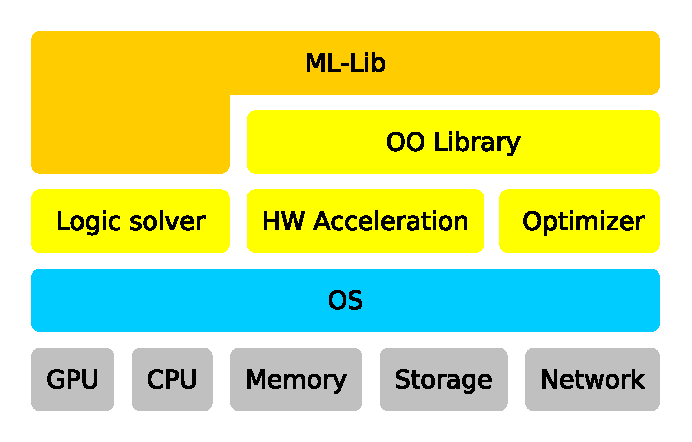
\includegraphics[width=\linewidth]{figures/layers.pdf}
        \end{column}
        \begin{column}{.65\linewidth}
            \begin{itemize}
                \item \alert{Library} of LP predicates\ldots
                \item \ldots for \alert{training/using} ML models
                \item Supports hybrid systems via \alert{ML + LP}
            \end{itemize}
        \end{column}
    \end{columns}
    %
    \prologimport{listings/hybrid-predictor.pl}
\end{frame}

\subsubsection{\twopkt{} for Inference}

\begin{frame}{\twopkt{}'s General API for Logic Resolution\ccite{2pkt-jelia2021}}

    \begin{columns}
        \begin{column}{.49\linewidth}
            \includegraphics[width=\linewidth]{figures/primitive-usage.pdf}
        \end{column}
        \begin{column}{.49\linewidth}
            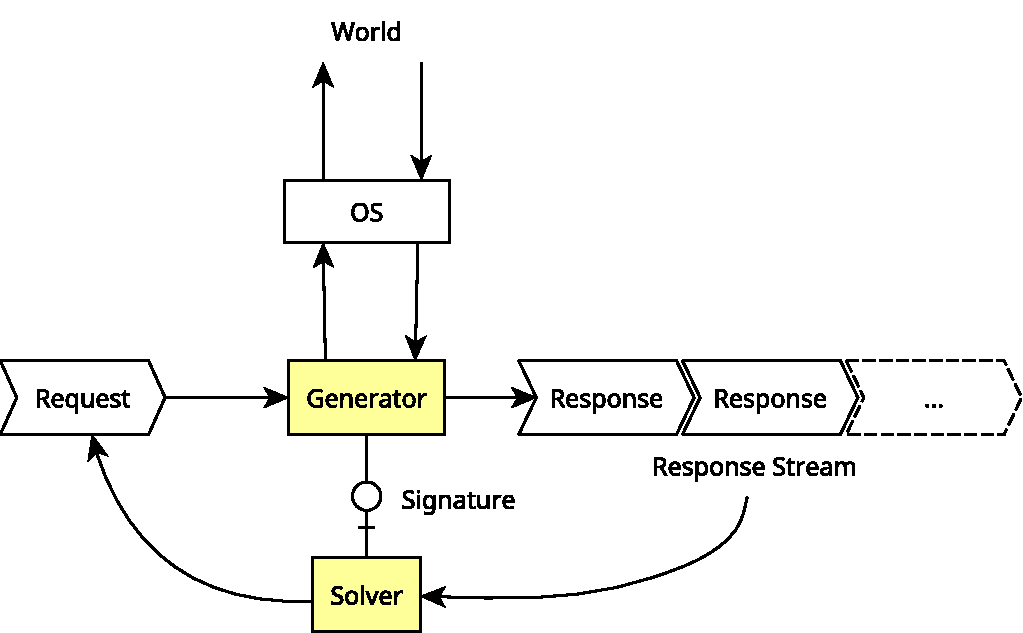
\includegraphics[width=\linewidth]{figures/generator.pdf}
        \end{column}
    \end{columns}

    \vfill

    \begin{itemize}
        \item Logic solvers as \alert{oracles} queried by users
        
        \vfill

        \item Generators as \alert{gateways} towards the external world
    \end{itemize}
\end{frame}

\begin{frame}{\twopkt{}'s support for Prolog-like Resolution\ccite{2pkt-jelia2021}}
    \begin{itemize}
        \item State-Machine for Prolog, proposed in \ccite{tuprolog-sac08}
        %
        \begin{itemize}
            \item extended to support \alert{generators}
        \end{itemize}
    \end{itemize}

    \begin{center}
        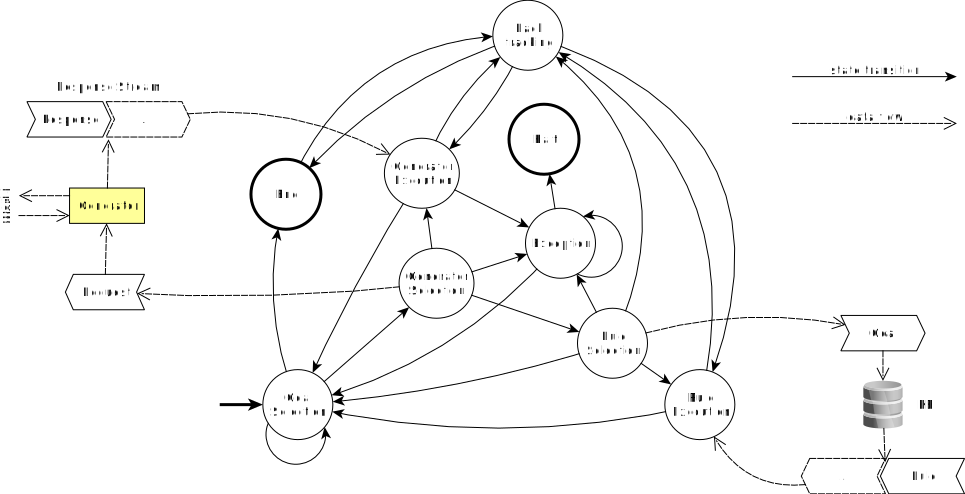
\includegraphics[width=.8\linewidth]{figures/2p-fsa-dataflow.pdf}
    \end{center}
    %
    \hfill\hint{formalization attempt here: \url{https://github.com/tuProlog/2pkt-state-machine}}
\end{frame}

\begin{frame}{\twopkt{}'s support for Probabilistic LP\ccite{dcc-aixia-2021-plp}}
    \begin{columns}
        \begin{column}{.49\linewidth}
            \fbox{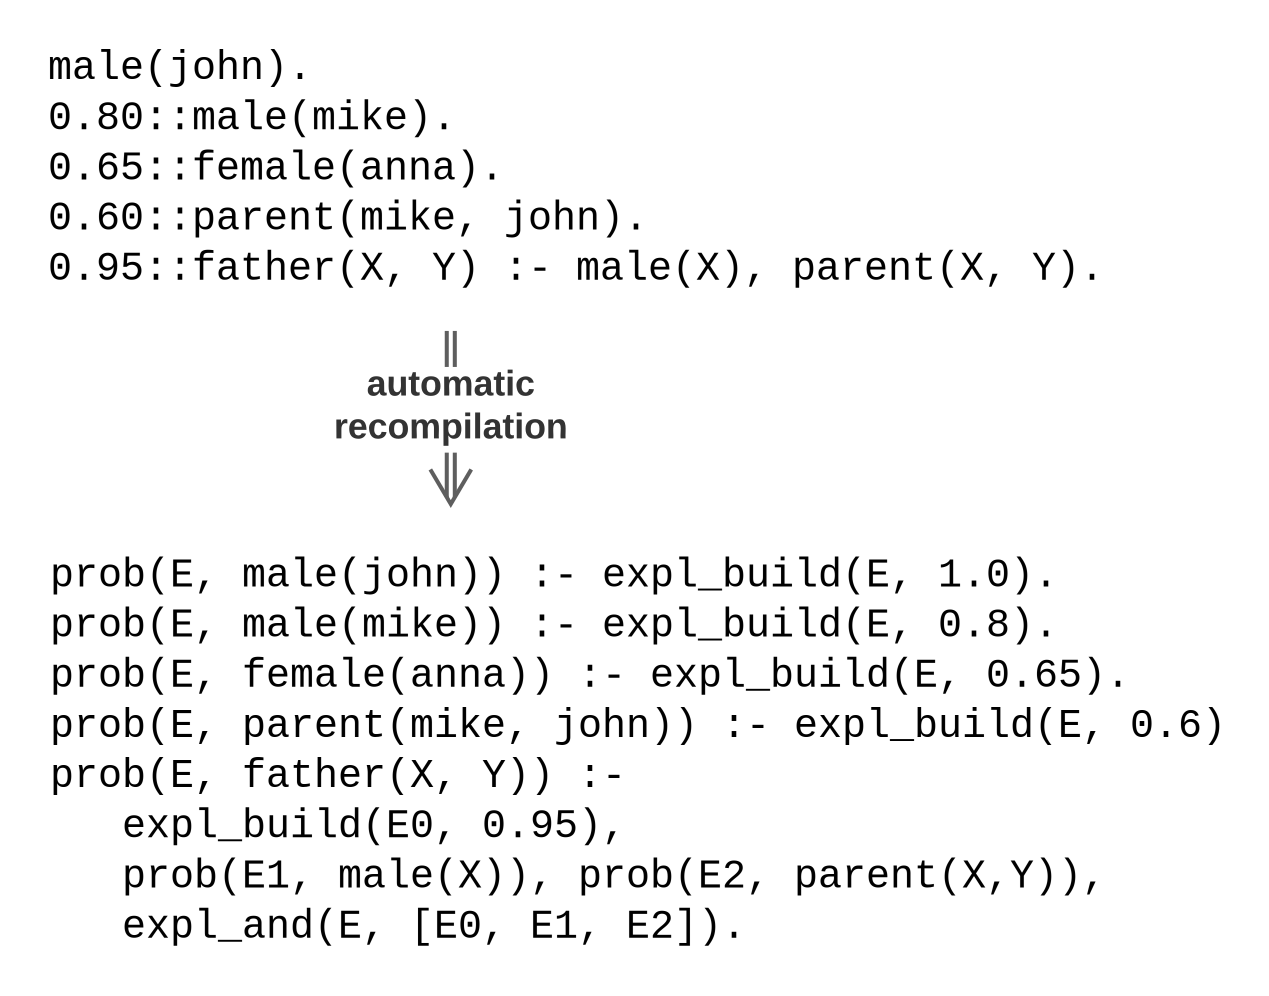
\includegraphics[width=\linewidth]{figures/design-problog-theory-transformation.pdf}}
        \end{column}
        \begin{column}{.49\linewidth}
            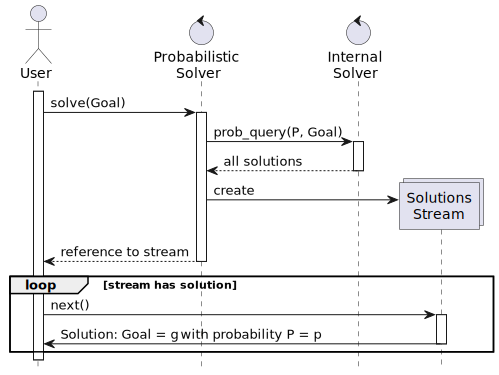
\includegraphics[width=\linewidth]{figures/general-api.pdf}
        \end{column}
    \end{columns}

    \vfill

    %
    \begin{itemize}\small
        \item Implementation of \alert{ProbLog}\ccite{de-raedt-2007}, based on \twopkt{}
        %
        \begin{itemize}
            \item supporting \alert{probabilistic}, fuzzy reasoning
        \end{itemize}
        \vfill
        \item Several tricks:
        %
        \begin{itemize}
            \item LPAD\ccite{VennekensVB04} programs \alert{converted} into Prolog
            \item extended Prolog solver exploited behind the scenes
        \end{itemize}
    \end{itemize}
\end{frame}

\begin{frame}{\twopkt{}'s support for Concurrent LP}
    \begin{itemize}

        \item Sketched in recent Master thesis\ccite{Giordano2021}

        \vfill

        \item Support for \alert{OR-concurrent} LP
        
        \vfill

        \item Based on \emph{modern} \alert{concurrent programming} facilities 
        %
        \begin{itemize}
            \item[eg] coroutines and fork-join pools
        \end{itemize}

        \vfill

        \item Immutable \& \alert{copy-on-edit} design to avoid synchronization overhead
    \end{itemize}
\end{frame}

\subsubsection{\twopkt{} for Explanations}

\begin{frame}{Platform for SKE based on \twopkt{} (\psyke{}\ccite{psyke-woa2021})}
    \begin{center}
        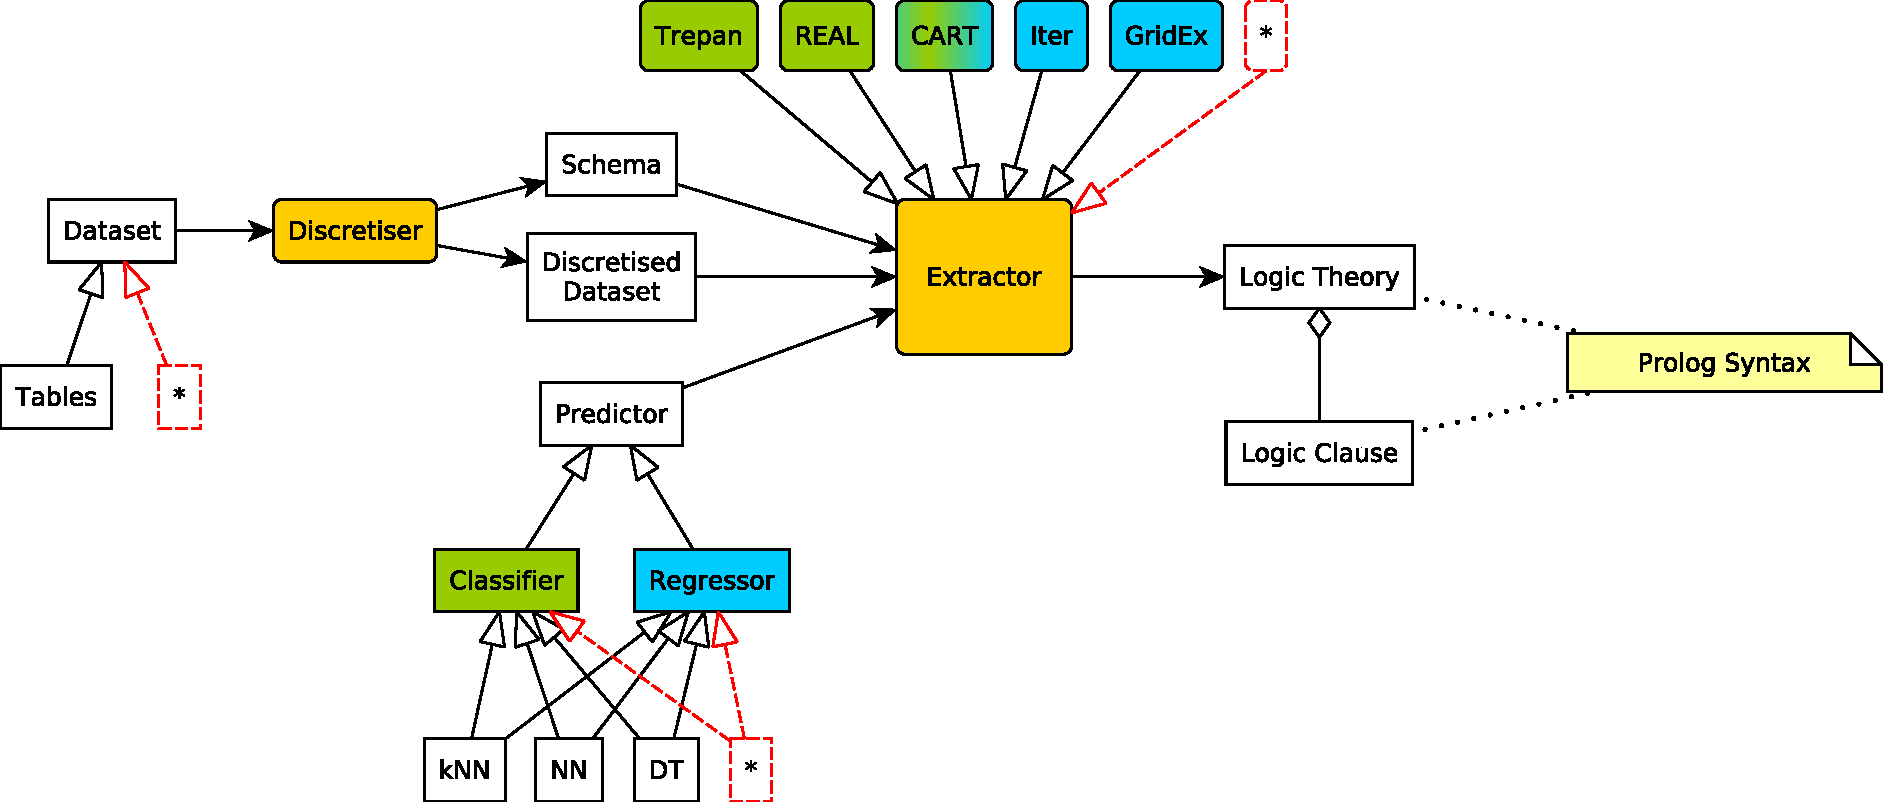
\includegraphics[width=.8\linewidth]{figures/Psyke.pdf}
    \end{center}
    %
    \vfill
    %
    \begin{itemize}
        \item general \alert{API} for \alert{SKE} out of ML models
        \vfill
        \item in the form of \alert{Prolog rules}
        \vfill
        \item via several extraction algorithms from the literature
        %
        \begin{itemize}
            \item plus some proposed by us\ccite{gridex-extraamas2021}
        \end{itemize}
    \end{itemize}
\end{frame}

%===============================================================================
\section{Conclusions and Future Works}
%===============================================================================

\begin{frame}{Summary of Contributions}
    \begin{block}{Computational perspective (what)}
        \begin{itemize}
            \item orthogonal approaches to knowledge representation
            \item analogous approaches to learning
            \item intuitive vs. rational approaches to inference
            \item logic as a means for explaining ML
        \end{itemize}
    \end{block}
    
    \begin{block}{Technological perspective (how)}
        \begin{itemize}
            \item lack of interoperable \& portable LBT 
            \item design and prototype the \twopkt{} ecosystem
            \item extend the ecosystem towards sub-symbolic AI, by supporting:
            %
            \begin{itemize}
                \item \alert{learning} via ILP and logic API for ML
                \item \alert{inference} via probabilistic and concurrent LP
                \item \alert{explanation} via \psyke{} 
            \end{itemize}
        \end{itemize}
    \end{block}
\end{frame}

\subsection{Future Works}

\begin{frame}{GNN as the Bridge among CL and ML\ccite{gnn-woa2021}}
    \centering

    \includegraphics[width=\linewidth]{figures/workflow.pdf}
\end{frame}

\begin{frame}{Symbolic Knowledge Injection\ccite{PsykiExtraamas2022, KinsCilc2022}}
    \centering

    \begin{figure}
        \begin{subfigure}{0.45\linewidth}\centering
            \fbox{\includegraphics[width=\linewidth]{figures/SKI-loss.pdf}}
            Constraining
        \end{subfigure}
        \hfill
        \begin{subfigure}{0.45\linewidth}\centering
            \fbox{\includegraphics[width=\linewidth]{figures/SKI-structuring.pdf}}
            Structuring
        \end{subfigure}
        
        \bigskip
        
        \begin{subfigure}{0.45\linewidth}\centering
            \fbox{\includegraphics[width=\linewidth]{figures/SKI-embedding.pdf}}
            Embedding
        \end{subfigure}
    \end{figure}
\end{frame}

\begin{frame}{Train-Extract-Fix-Inject (TEFI) Loop}
    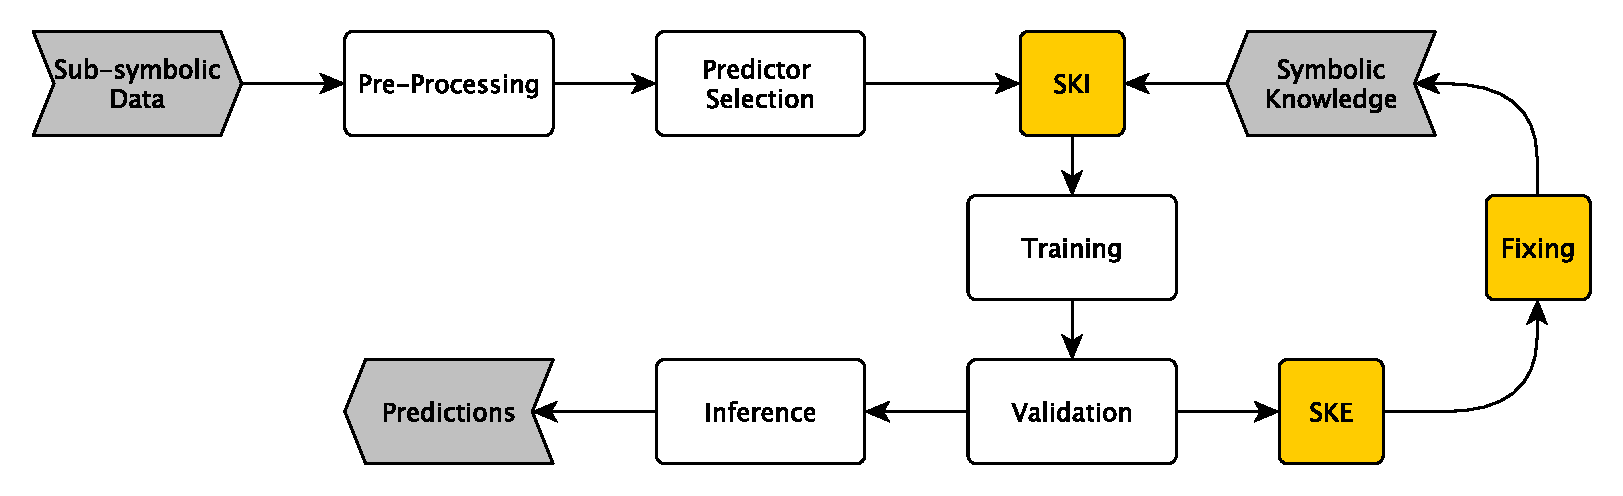
\includegraphics[width=\linewidth]{figures/train-extract-fix-inject.pdf}
\end{frame}

%===============================================================================
\section*{}
%===============================================================================

%/////////
\frame{\titlepage}
%/////////

%===============================================================================
\section*{\refname}
%===============================================================================

%%%%
\setbeamertemplate{page number in head/foot}{}
%/////////
% \begin{frame}[c,noframenumbering]{\refname}
\begin{frame}[t,allowframebreaks,noframenumbering]{\refname}
%	\tiny
    \scriptsize
%	\footnotesize
    \bibliographystyle{apalike-AMS}
    \bibliography{phd-defense,my-papers}
\end{frame}
%/////////

%%%%%%%%%%%%%%%%%%%%%%%%%%%%%%%%%%%%%%%%%%%%%%%%%%%%%%%%%%%%%%%%%%%%%%%%%%%%%%%%
\end{document}
%%%%%%%%%%%%%%%%%%%%%%%%%%%%%%%%%%%%%%%%%%%%%%%%%%%%%%%%%%%%%%%%%%%%%%%%%%%%%%%%
